
\chapter{=================}
  \textcolor{yellow}{===========================}
\chapter{=== Drafts ===}

\section{0000}  


\subsection{0000}  {
% ~~~~~~~~~~~~~~~~~~~~~~~~~~~~~~~~~~~~~~~~~ %
% ~~~~~~~~~~~~~~~~~~~~~~~~~~~~~~~~~~~~~~~~~ %
% ~~~~~~~~~~~~~~~~~~~~~~~~~~~~~~~~~~~~~~~~~ %
% ~~~~~~~~~~~~~~~~~~~~~~~~~~~~~~~~~~~~~~~~~ %

 
\textcolor{green}{Fix 一個 unit system,觀察 piece 的變化就好 }
\begin{figure}
    \centering
    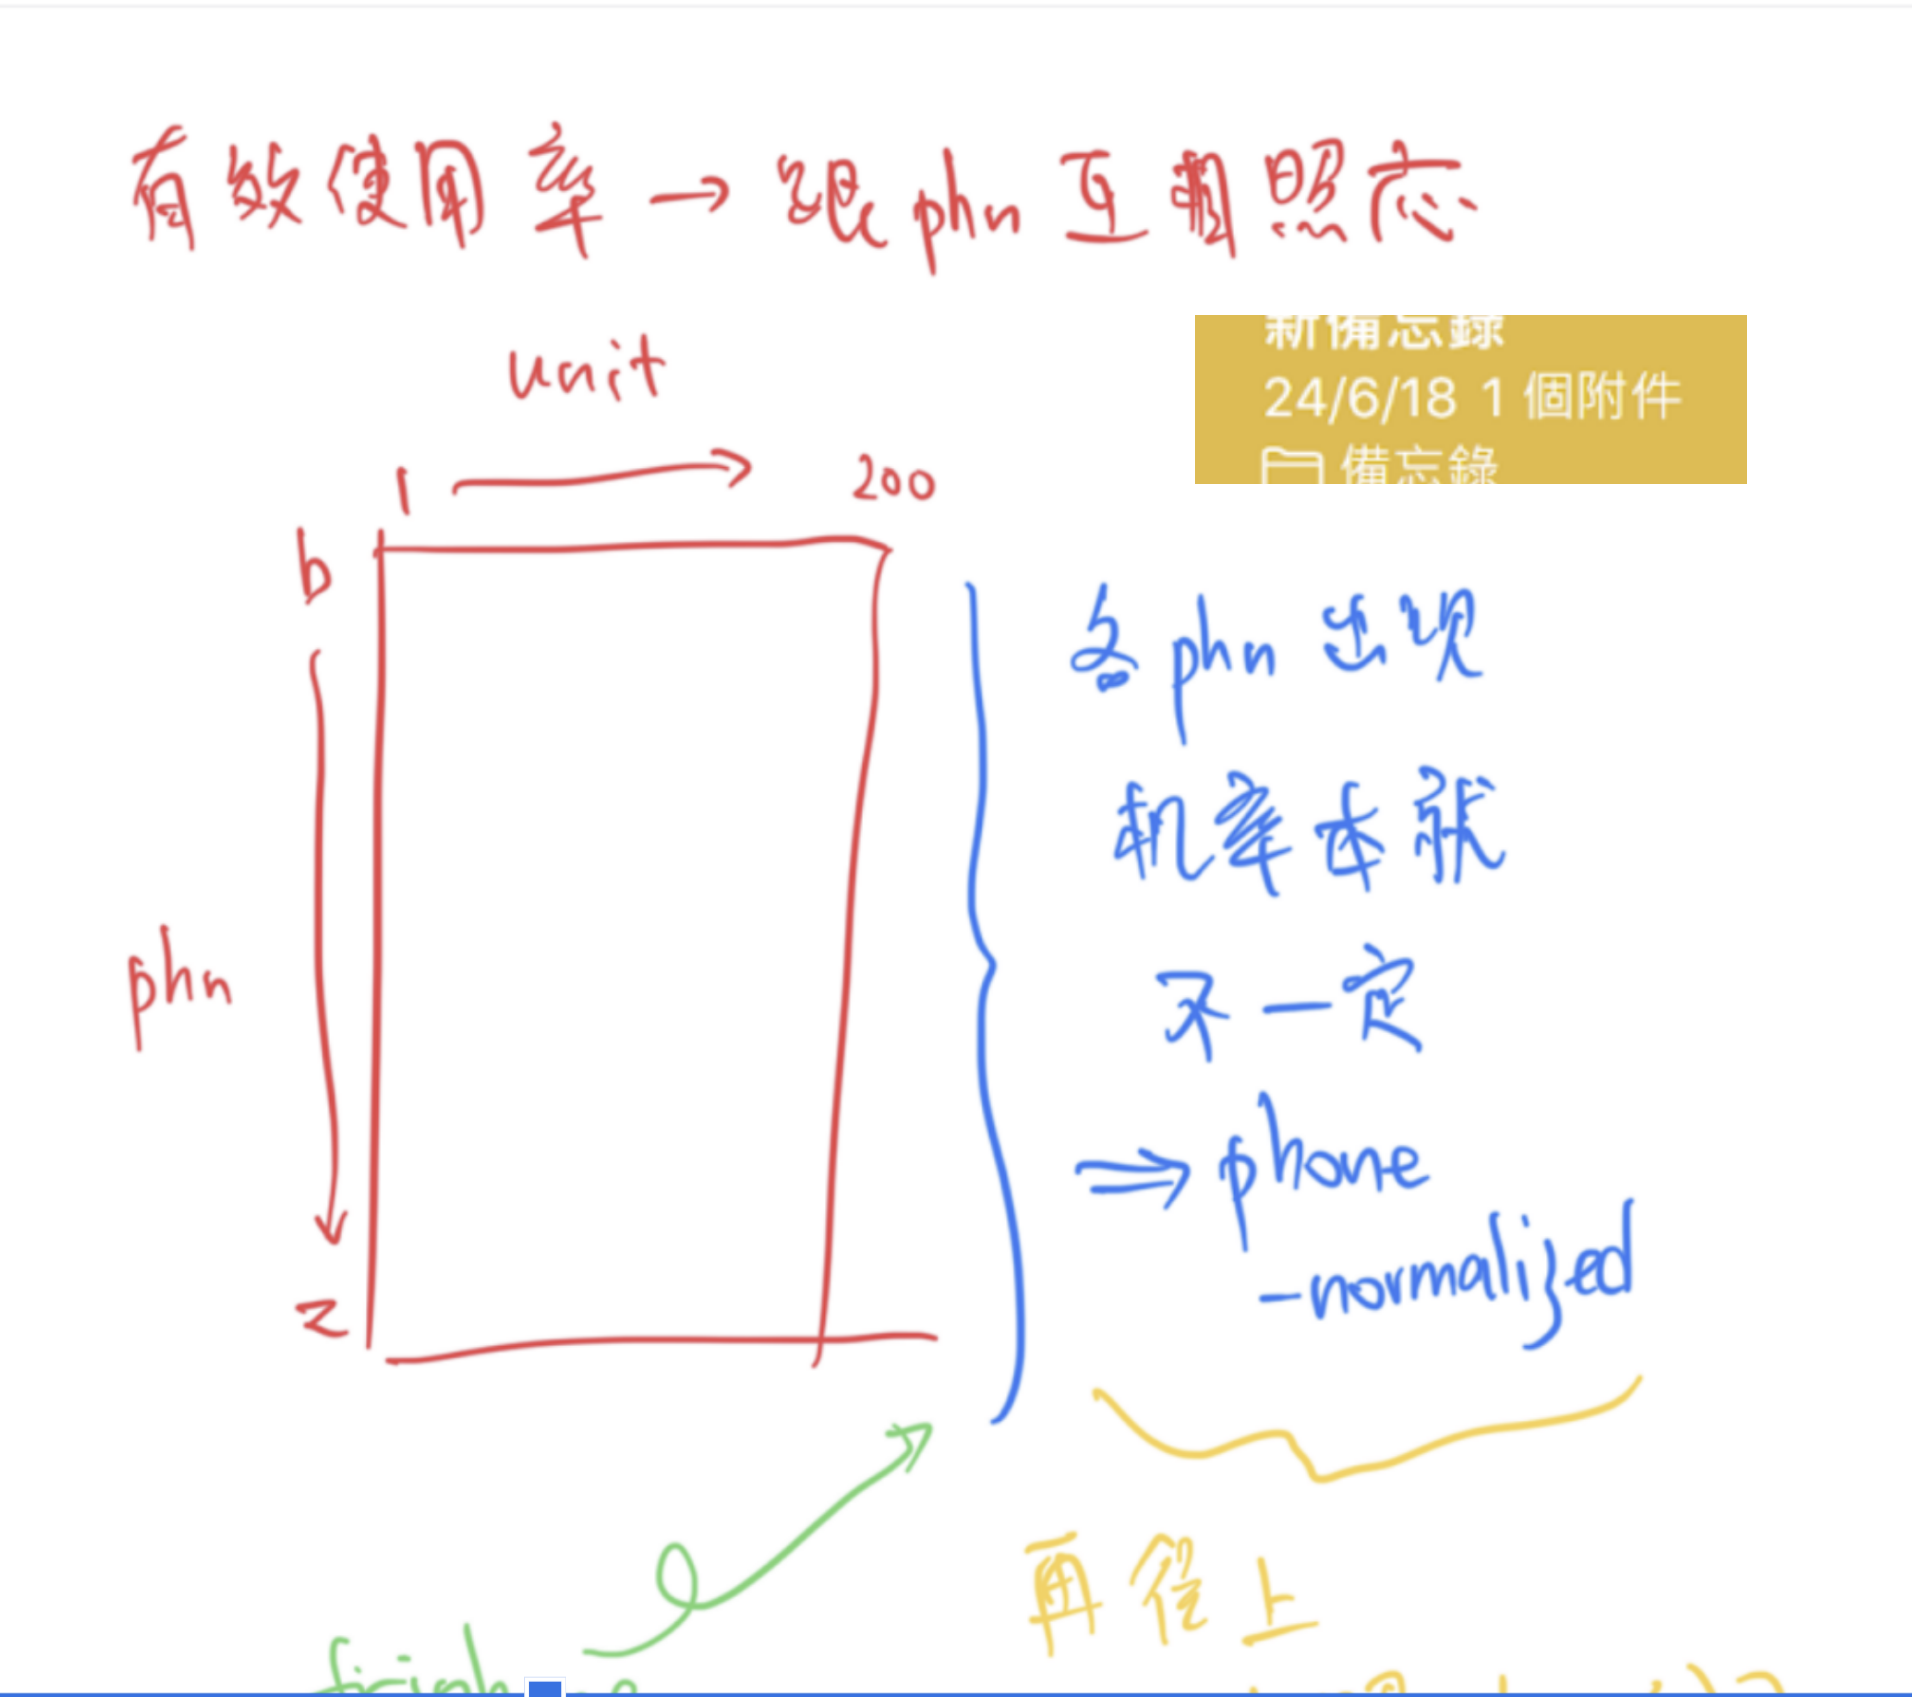
\includegraphics[width=1\linewidth]{feasiblefigs/ch4figs/drafts/0.png}
\end{figure}
}
 %%%%%%%%%%%%%%%%%%%%%%

\mychcnt{4}\chapter{●}\section{●}  % ====== %  ●●

  \textcolor{magenta}{------------------------------------------------}
\mychcnt{4}\chapter{●}\section{●}  % ====== %  ●●
\subsection{Ch3}
\begin{enumerate}
    \item 熱圖 → $\pi$
    \item unit
      \begin{itemize}
        \item $H_u(\varphi)$ 高低分佈
        \item $Pr_u(\varphi)$→ 其他 phn 語音關係
        \item $\pi'$ (驗證關係)
      \end{itemize}
    \item phn
      \begin{itemize}
        \item $H_{\varphi}(u)$ → 發音特性
        \item $\pi_{類}$ → 比較類別
      \end{itemize}
    \item 整體 → 模型 & 發音
\end{enumerate}
{
% ======================== %
\subsection{Ch4}
\begin{itemize}
    \item (我要不要補上 BPE worse than natural more units? --> but KMeans 耗費,但 BPE 就不?)
    \item %
\end{itemize}

\subsection{Dh4 -- Multiunits}  % 介紹 & 跑
\begin{enumerate}
    \item 介紹 subwords
    \item 何以分析 & 結果
\end{enumerate}

          % =============== %          
---------------------------------------------------
{
\cite{-}  % =============== %   - ✔️
}
% ======================== %
}
